\documentclass[authoryear, review,12pt,number]{elsarticle}
%\documentclass[authoryear, preprint,12pt,number]{elsarticle}
\usepackage[utf8]{inputenc}
\usepackage[T1]{fontenc}
\usepackage[numbers]{natbib}
\usepackage{graphicx}
\usepackage{float}
\usepackage{rotating}
\usepackage{stfloats}
\usepackage{lineno}
\usepackage[linesnumbered,ruled,vlined]{algorithm2e}
\usepackage{tabulary}
\usepackage{graphicx}
\usepackage{color}
\usepackage[none]{hyphenat} \usepackage[table]{xcolor} \sloppy
\usepackage{hyperref}
\usepackage{amsmath}
\usepackage{multirow}
\usepackage{rotating}
\usepackage{adjustbox}
\usepackage{graphicx}% http://ctan.org/pkg/graphicx
\usepackage{booktabs}% http://ctan.org/pkg/booktabs
\usepackage{xparse}% http://ctan.org/pkg/xparse
\usepackage{booktabs}
\usepackage{array}
\usepackage[ddmmyyyy]{datetime}
\usepackage{listings}
\renewcommand{\dateseparator}{.}

\newcolumntype{R}[2]{%
    >{\adjustbox{angle=#1,lap=\width-(#2)}\bgroup}%
    l%
    <{\egroup}%
}
\newcommand*\rot{\multicolumn{1}{R{60}{1em}}}% no optional argument here,
% please!
\begin{document}
\begin{titlepage}
\begin{center}

% Upper part of the page. The '~' is needed because \\
% only works if a paragraph has started.
\textsc{\LARGE Technische Universit\"at Berlin}\\[0.5cm]
\textsc{Master Thesis}\\[1.5cm]

\textsc{\Large Classifying EUNIS Habitats using Ontologies and Data Mining
Methods}\\[1.5cm]
\textsc{\textit{A thesis submitted in partial fulfillment of the requirements
for the degree of}}\\[1.25cm]
\textsc{\Large Master of Science in Environmental Planning}\\[1.5cm]
\textsc{Faculty VI - Planning Building Environment\\
 Geoinformation in Environmental Planning}\\[1.5cm]

% Title
% Author and supervisor
\noindent
\begin{minipage}{0.5\textwidth}
\begin{flushleft} \large
\emph{Author:}\\
T. Niklas \textsc{Moran}
\end{flushleft}
\end{minipage}%
\begin{minipage}{0.5\textwidth}
\begin{flushright} \large
\emph{Supervisor:} \\
Prof. Dr.~Birgit \textsc{Kleinschmit}
Mag. rer. nat. ~Simon \textsc{Nieland}
\end{flushright}
\end{minipage}

\vfill

% Bottom of the page
{\large December 2015}

\end{center}
\end{titlepage}

\begin{titlepage}
\begin{center}
{Author's Declaration}
\end{center}
I hereby certify that I am the sole author of this master thesis. 
Furthermore, I confirm that no sources have been used in the preparation of this thesis other
than those indicated in the thesis itself. The works of other people included in
my thesis, published or otherwise, are fully acknowledged in accordance with the
standard referencing practices. This thesis has not been submitted for another
degree or master to any other University or Institution.
\\
\\
Hiermit versichere
ich, dass ich die vorliegende Arbeit selbstst�ndig verfasst und keine anderen als die
angegebenen Quellen und Hilfsmittel benutzt habe. Alle Ausf�hrungen, die anderen
ver�ffentlichten oder nicht ver�ffentlichten Schriften w�rtlich oder
sinngem\"a\ss entnommen wurden, habe ich kenntlich gemacht. Die Arbeit hat in
gleicher oder \"ahnlicher Fassung noch keiner anderen Pr\"ufungsbeh\"orde vorgelegen.

\vfill
\begin{center}
\noindent
\begin{minipage}{0.5\textwidth}
\begin{flushleft}
\rule{5cm}{0.4pt}
Date/Datum 
\end{flushleft}
\end{minipage}%
\begin{minipage}{0.5\textwidth}
\begin{flushright} 
\rule{5cm}{0.4pt}
Signature/Unterschrift
\end{flushright}
\end{minipage}


\end{center}
\end{titlepage}

\begin{frontmatter}
\linenumbers
\title{Classifying EUNIS habitats using ontologies and data mining methods}

\author[TUB]{T. Niklas Moran\corref{cor1}}
\ead{niklasmoran@mailbox.tu-berlin.de}

\author[TUB]{Simon Nieland}
\author[TUB]{Birgit Kleinschmit}

\address[TUB]{Geoinformation in Environmental Planning Lab, Technische
Universit\"at Berlin, Stra\ss e des 17. Juni 145, 10623 Berlin, Germany}

\cortext[cor1]{Corresponding author at: Geoinformation in Environmental Planning
Lab, Technische Universit\"at Berlin, Stra\ss e des 17. Juni 145, 10623 Berlin,
Germany}

\begin{abstract}
  Remote sensing Biodiversity monitoring and 
\end{abstract}

\begin{keyword}
remote sensing, biotope classification, data mining, nature conservation, OWL, EUNIS, GEOBIA
\end{keyword}
\end{frontmatter}
\linenumbers

\section{Introduction}
Recognizing the importance of functioning habitats to reduce biodiversity loss,
the European Union has implemented an environmental conservation framework to
protect and conserve vital habitats in accordance with the Convention on
Biological Diversity. An integral part of this framework is the EU Habitats
Directive (Council Directive) 92/43/EEC [1992], which established the Natura
2000 network of habitats. The directive requires conservation and monitoring of
designated habitats by member states and for a report to be submitted every six
years. Environmental data to determine biodiversity status must be collected to
comply with the statute. Yet, comparing data used for these reports is difficult
due to varying data collection methods and aquisition nomenclatures by the
nature conservation authorities in each member state \citep{VandenBorre2011}.
The main issue lies in the subjective nature of field surveys to identify
habitats \citep{Cherrill1999, Cherrill1999a, Hearn_2011, Nieland2015}.
Furthermore, habitat status is mostly generated in bottom-up approaches taking
into account the national and regional interpretation guidelines
\citep{VandenBorre2011, INSPIREdataspecs}. This subjective and time-consuming
task of conducting field surveys could be partially replaced with an automated
remote sensing (RS) method that uses Geographic Object-Based Image
Analysis(GEOBIA) to reduce subjectivity, costs and time.
\\
Remote sensing offers opportunities to collect and automatically interpret large
amounts of computer-readable data useful for nature conservation and
biodiversity monitoring \citep{Corbane2015, VandenBorre2011, Mayer2011}. RS
image analysis implicitly incorporates the expertise of the person performing
the analysis, reducing reproducibility as the analyst ultimately chooses class
membership in non-crisp boundaries between classes. This can be divided into
remote sensing knowledge (spectral signature, remote sensing indices, etc.) and
field knowledge (feature properties, spatial relations, etc)
\citep{Andres2013a}, which is often neither completely nor explicitly defined as
it is based on trial and error but influences the classification
\citep{Arvor2013}. To ensure accuracy and applicability of classification
outputs for conservation, experts with detailed knowledge of the sites are
needed to interpret the RS data. The distance between the high-level semantics
used by experts to describe domain concepts and the low-level information
quantified from data is referred to as the ``semantic gap''.
\\
Ontologies can help bridge the ``semantic gap'' and allow for better data
transferability, predictability, interchangeability, knowledge and workflow
management (provenance) and logical consistency \citep{Janowicz2012}.  The
standards-compliant format designed and adopted to express rich semantics and
enable the ``Semantic Web'' is called the Web Ontology Language
(OWL2)\footnote{\url{http://www.w3.org/TR/owl2-overview/}}. The format supports
multiple syntaxes yet defines the Resource Description Framework (RDF)/XML
(subject, predicate, object triplets) as a common exchange format.
\\
Moreover, through the use of reasoners (inference engines) that infer logical
consequences over axioms and asserted facts and verify consistency, one can
discover new knowledge \citep{Arvor2013, Andres2013a}
RS and field expert
knowledge can be digitized in ontologies, thus allowing for a hierarchy of
concepts for improved automatic image annotation and retrieval using concepts
from both fields to produce more accurate results \citep{Srikanth_2005}.
Janowicz \cite{Janowicz2012} advocates for more observation-driven ontologies and for
including machine learning, statistics and data mining to construct ontological
primitives. While published research on using observation-based ontologies for
biotope classifications is limited, the available research using ontologies in
RS research is briefly summarized below.\\
Ontologies modeled on the Land Cover Classification System and the General
Habitat Category were integrated into tools used to monitor and protect areas in
the EU \citep{Arvor2013}. The authors note that using the taxonomy of the
different classification systems makes it possible to include expert knowledge
in the process. 
%Further research included expert knowledge from remote sensing
%and ecology to classify Natura 2000 sites using a hierarchical classification
%system. %hier fehlt eine Quelle!
\cite{Lucas2015} used pixel-based analysis and OBIA for greater classification
accuracy which relies on a rule-base created by an expert. Other research
includes classification of urban building types using a three-layered
architecture \citep{diSciascio2013} and a semi-automated classification of urban
building using the Random Forest (RF) classifier to determine variable
importance of features from airborne laser scanner data \citep{Belgiu2014}.
Ontologies have also been paired with different algorithms to automatically
acquire classification rules: a genetic programming algorithm
\citep{Forestier2012470} and the C4.5 data mining algorithm
\citep{Sheeren2006ML}. In biodiversity monitoring research, ontologies have been
demonstrated to improve spatial data interoperability by \cite{Nieland2015} and
a habitat quality tool showing trends and indicators led to the discovery of
relationships between phenomena \citep{Perez-Luque2015}. 
\\
The addition of fuzzy data types to OWL2 and the development of a fuzzy spatial
reasoner holds great promise for the future of GEOBIA ontology research using
remote sensing \citep{Bobillo2011, Bobillo2015}. More recently a multi-scale
fuzzy spatial reasoner was developed which could have significant impact on this
research \citep{Argyridis2015}.
\\
Even though researchers recently developed a number of indicators using
different sensors for habitat evaluation \citep{Nagendra2013}, classification
procedures and rule-sets were not formalized to be computer readable and
therefore suffer from similar transferablity and reproducibility problems as
manual habitat mapping \citep{Arvor2013, Nieland2015}. Therefore a formalized
computer-readable ontology could help solve these problems and allow scientists
to see how the classification was performed and be aware of possible
incompatibilities before combining data \citep{Janowicz2012}.  Furthermore,
there is no standardized set of indicators using RS for trans-national habitat
evaluation \citep{Lucas2015, VandenBorre2011}. Therefore, technical solutions to
increase interoperability by thematically harmonizing environmental data and
systematize data collection methods from remote sensing inputs in an automated
workflow are needed. 
\\
The EIONET Action Group on Land monitoring in Europe (EAGLE) is an expert group
that seeks to harmonize land cover (LC) and land use (LU) nomenclatures using an
object-oriented data model that eases translations between nomenclatures
\citep{arnold2013eagle}. The many different nomenclatures used in Europe each
have their own specific thematic conceptualization suited towards a specific
scale and data collection method- reducing the ability to compare thematic maps.
Since LU and LC are interconnected and influence one another, nomenclatures
often incorporate both definitions into one class making separation difficult.
To overcome this problem the EAGLE data model describes landscapes in three main
components: land cover (abiotic, vegetation, water) land use (agriculture,
forestry, etc.) and characteristics (bio-physical, cultivation etc). The
increased interoperability and transferability of RS data and the semantic layer
on top helps decision-makers to better assess and compare outcomes. 
\\ 
In this paper we propose an automated system that can classify dry, mesic and
wet grassland habitats according to the European Union Nature Information System
(EUNIS) biotope classification schema using earth observation data, existing
thematic maps (biotope, forestry, etc.), and expert knowledge formalized in an
ontology by taking into account rules generated by data mining algorithms. The
combination of data mining algorithms with ontology-based classification has, to
our knowledge, not yet been done and is a first in remote sensing research. 
This method contributes to the goal of empirically-derived rule creation and enhances data interoperability and
comparison as proposed \cite{Janowicz2012}.
The main goals of this paper are:
\begin{itemize}
 % Birgit wird data mining sagen statt machine learning- ich finde die begriffe
 % ziemlich aenlich!
 % using advances in artificial intelligence?
 \item to develop a RS classification methodology using data mining approaches
     in combination with ontological formalism to generate highly interoperable,
     reproducable and exchangeable classification procedures and results,
 \item apply the methodology to indicators used to separate grassland habitats
     defined under EUNIS
 \item and evaluate the developed approach by comparing it to a state-of-the art
     machine learning classifier (Extra Tree Classifier\footnote{link zur
     website})
\end{itemize}

%We use EAGLE concepts to overcome these issues and ease translation/application
%to a different domain. Das kommt wieder in die Methode
%An OWL2 ontology is composed of classes, individuals 
%and properties. Classes are sets of individuals and properties come in 
%two forms: an object property defines a relationship between two individuals 
%and a data property  places a data type constraint on the 
%individual \citep{OWL2}. Das klingt nach Methode. Runter oder raus.
\section{Use case: Classifying EUNIS grassland habitats in
Rhineland-Palatinate}
%hier würde ich ein paar Einleitende Worte schreiben. Dass wir unsre Methodik
% testen wollen an und dafür folgenden use-case ausgewählt haben.
\label{subsec_data_study_area}
Saarburg is an 200km$^{2}$ administrative district and is located in the
south-west of the federal state of Rhineland Palatinate (RLP), Germany.
Luxembourg borders the area to the west and the federal state of Saarland to
the South. RLP has a western european atlantic climate and has an economically
and culturally important viticulture industry along the Mosel and Rhine rivers.
%hast du ganz Saarburg als Testgebiet genommen? Vielleicht kannst du noch die
% Anzahl der Grünlandflächen dazu schreiben.
\begin{figure}
\label{fig_study_area}
    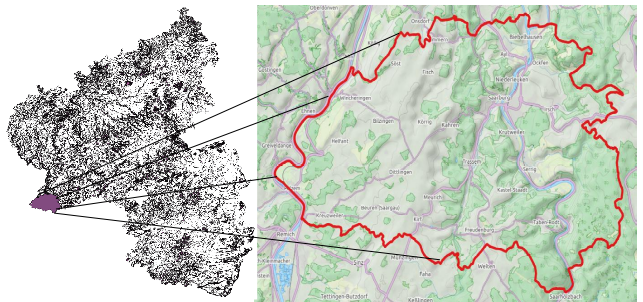
\includegraphics[width=\textwidth]{diagrams/study_area_closeup.png}
    \caption{Saarburg is purple location Saarburg in purple in relation to
    Rheinland Palatinate. Map on right \copyright Thunderforest, Data
\copyright OpenStreetMap contributors.}
\end{figure}


\subsubsection{Target indicators and base nomenclatures}
\label{subsec_target_indicators_nomenclatures}
We tested our method on dry, mesic and wet grasslands (EUNIS classes E1, E2 and
E3 respectively). We adapted the selected EUNIS indicators to meet the
requirements of remote sensing analysis. We also adopted the EAGLE
object-oriented approach by separating LU, LC and characteristics and adopted 
terms when possible to increase interoperability and further re-use. The table
~\ref{tab_indicators_classes} shows the list of indicators that can be detected
by our data and aggregated to form EUNIS classes. 
\begin{table}
\centering
  \begin{tabular}{clcccccccc}
  \rot{description}&\rot{EUNIS class}&\rot{wetness} & \rot{vegetation type} &
  \rot{usage} & \rot{usage intensity} & \rot{immature
  soil} & \rot{hydromorphic} & \rot{species richness} \\ \hline
\multirow{3}{*}{dry}
    & E1   & dry & g/h & g/m/- & low & 1 & 0 & 0/1/- \\ 
    & E1.2 & dry & g/h & g/m/- & low & 1 & 0 & 1\\
    & E1.7 & dry & g/h & - & low & 1 & 0 & -/0\\ 
\multirow{4}{*}{mesic} 
    & E2   & mesic & g/h & g/m/- & l/m/h/- & 0 & 0 & 0/1/-\\
    & E2.1 & mesic & g/h & g & medium/high & 0 & 0 & -/0/1 \\
    & E2.6 & mesic & g & g/m/- & high & 0 & 0 & 0 \\
    & E2.7 & mesic & g/h & - & - & 0 & 0 & 0/1/- \\
\multirow{3}{*}{wet}
    & E3   & very wet & g/h & g/m/- & low/medium & 0 & 1 & 0/1/- \\
    & E3.4 & very wet & g/h & g/m & medium & 0 & 1 & 0/1 \\
    & E3.41 & very wet & g/h & m & medium & 0 & 1 & 1 \\
\end{tabular}
\caption{A `/ ' denotes OR and a '-' denotes 'none' and the first letter of 
each value is used to safe space. Vegetation type: {graminaceous, 
herbaceous}, usage: {grazing, mowing}, usage intensity: {low, medium, high}. 
}
\label{tab_indicators_classes}
\end{table}
\subsubsection{Data}
For the pre-segmentation step (see
\ref{subsec_Preparation_of_reference_data_and_semantic_characterisation}) two
types of data bases were taken into account. Digital orthophotos (resolution
???) are used to create the Digital Surface Model (DSM) using automated stereo
matching and therefore represent the basis for all segmentation and
classification procedures. The DTM and DEM was produced using LiDAR ASCII point
clouds acquired between 2003 and 2009 with a resolution of 0.2m.\\

The reference data (see
\ref{subsec_Preparation_of_reference_data_and_semantic_characterisation})
consists of the federal biotope map (paritally updated 2015), a federal
agriculture dataset (INVEKOS updated every year) and a soil map (resolution xxx)
which is based on the ALKIS (Amtliches Liegenschaftskaster
Informationssystem?!).
%Die Walddaten kannst du raus lassen. Die hast du ja fuer die Arbeit nicht
% benutzt.
The actual classification process is based on two RapidEye Scenes (Year:xx and
yy) and indices of the DTM, DEM and orthophotos.


\begin{figure} 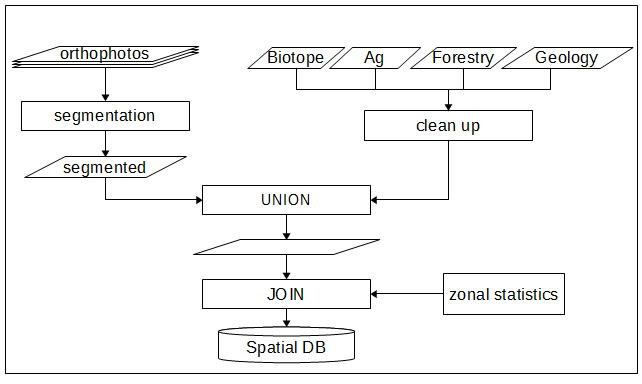
\includegraphics[width=1\textwidth]{diagrams/pre_processing.png}
    \caption{Biotope, Agriculture, Forestry, Geology (soil maps) are combined 
    (union) and joined with the segmented polygons (derived from orthophotos) 
    fitting within the combined polygons. The features are joined together 
    and get all properties associated from the dataset unless they conflict. 
    When conflicts occur the corresponding column is marked as such.}
\label{fig_pre-processing}
\end{figure}

\section{Method}
This section describes the developed method for ontology-based, multi-source
classifying of EUNIS habitats.
%Die Datenaufbereitung muss ebenfalls noch besser beschrieben werden.
\label{subsec_method_overview}
\subsection{Overview of the automated EUNIS Habitat Mapping System}
 Figure ~\ref{fig_full_workflow} gives an overview of the method using the
 wetness indicator as an example of one of the habitat indicators needed to
 differentiate dry, mesic and wet grassland habitats according to level 2 of
 EUNIS. 
% The developed system is comprised of (1) attaching formalized indicators
% (section \ref{subsec_formalization_expert_knowledge}, Table
% \ref{tab_indicators_classes}) from expert knowledge to polygons created during
% the segmentation step, (2) rule generation by running data mining algorithms
% over randomly selected polygons using the habitat indicators as class labels
% (\ref{subsec_rulegen_data_mining})
% (3) importing rules, EUNIS classes
% and polygon attributes into an ontology and finally
% (\ref{subsec_rulegen_data_mining}) (4) classifying polygons
%with the Fact++ reasoner \citep{Tsarkov2006} and writing results back to the
%database. 
%Die Beschreibung stimmt nicht mit der Graphik ?berein!
The developed system is comprised of (1) the preparation of reference data,
including a spatial union of the base data sets (pre-segmented,
pre-classified areal photos and thematic maps (see \ref{data_reference}) and the attachment
of subsequent semantic characteristics (see \ref{data_reference)}, (2) the
selection of training and validation data (see \ref{validation}), (3) the
generation of classification rules taking into acount different machine
learning algorithms and finally (4) the ontology-based classification process
(see \ref{classification}).
\label{subsec_software}
\subsubsection{Software Overview}
The software relies on a PostgreSQL database and various open source Python and 
Java libraries to interact with the database, convert files and execute a 
reasoner over the created OWL file.
The OWLAPI \footnote{\url{https://github.com/owlcs/owlapi}} is used to interact 
with the OWL files and execute the FaCT++
reasoner \citep{Tsarkov2006}. Currently the rule generation module uses two 
algorithms %from scikit-learn müsstest du voher einführen. Mach lieber
% footnotes! oder Zitate
: decision tree classifier (DT) and one additional algorithm called the Separability and 
Thresholds (SEaTH) algorithm \citep{Nussbaum2006}. The and tree 
classifier (ET) %footnote
is performed as reference classification
%% where does this paragraph go?! good question! ;-)

% The SEaTH algorithm statistically identifies characteristic features and their
% thresholds. It has been used on remote sensing data for land cover
% classification \citep{Gao2011, Mhangara2013} and nuclear installation
% classification \citep{Nussbaum2006}.  The DT is a modified classification an
% regression tree (CART)\citep{scikit-learn}. CART has been used in many MODIS and
% Landsat TM studies and is used in the standard MODIS land cover data
% \citep{friedl2002global}. Many remote sensing studies use it and it performs
% well in classification tasks \citep{Li_2014, Qian_2014, Shao_2012}.
% %%% Dieser Absatz muss, wenn überhaupt, in die Einleitung
%The data mining module is described in the next section
% \ref{subsec_rulegen_data_mining}.% Data mining module gibt es so in der
% Graphik nicht. raus!
%______________________
% 
% After the algorithms produce rules for each indicator, these are then added as
% facet restrictions to an OWL ontology.  The polygons from the testing table are
% loaded from the database as OWLIndividuals into the same ontology and the
% reasoner FaCT++ classifies all polygons according to the rules. The
% classification results by the reasoner is written to the database. The full
% workflow is shown in figure 
% \ref{fig_full_workflow}. => das muss zur classification


%Diesen Teil musst du noch genauer
% beschreiben. Das ist der Kern deiner Arbeit. Auch wenn du dich in den n?chsten
% Unterkapiteln nochmal wiederholst. Es ist sehr wichtig f?r das Verst?ndnis,
% dass du hier alles detalliert beschreibst. Ich w?rde f?r jeden Punkt
% mindestens einen Satz schreiben.
% Verweise auf die anderen Kapitel (z.b. (1) ist beschrieben in 2.2 und 2.3 
% Hier muss noch rein: Woher kommen die
% Ausgangsdaten? Wie wurden Referenzdaten erstellt?(Verweise auf Kapitel 2.2)
% Wie funktioniert das Sampling? Wie formalisierst du die Regeln (OWL Axioms)?
% Schreibe, dass wetness in der Graphik nur ein Beispiel ist und du das f?r
% verschieden Indikatoren anwenden willst. Erkl?re A-Box und T-Box reasoning.
%Erkl?re Expert knowledge. Wer macht da was? 
\begin{figure}
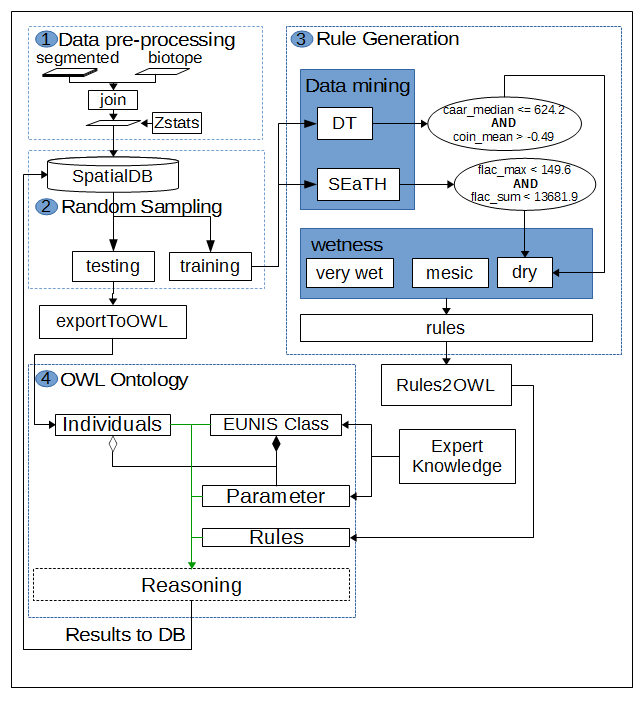
\includegraphics[width=1\linewidth]{diagrams/another_workflow_diagram_large.png}
\caption
    {
        1) The thematic maps (biotope, forestry, etc.) are joined together and
        statistics are calculated for each combined polygon.
        2) Training and testing data are created and saved in the database.
        3) The training data is loaded into the data mining module and the
        rules are generated for e.g.\ the ``wetness" indicator
        4) The rules are imported into the OWL ontology along with the testing
        data as individuals. The reasoner performs A-box reasoning to determine
        class membership.
    } 
\label{fig_full_workflow}
\end{figure}
%Generell ist das Kapitel noch sehr durcheinander! Ich w?rde mich von hier an
% einfach an die Struktur aus der ?bersicht halten! d.h. 
% 2.2 Preparation of reference data and semantic characterisation
% 2.3 Selection of training/validation data
% 2.4 Rule generation
% 2.5 Formalisation and ontology-based classification 
% 2.6 Validation
% 2.7 Use-case: Classification of EUNIS grassland habitats in
% Rhineland-Palatinate

%Ich versuchs mal:

%subsubsections kommen sp?ter raus: Ich hab sie nur drin gelassen um den
% ?berblick zu behalten


\label{subsec_Preparation_of_reference_data_and_semantic_characterisation}
\subsection{Preparation of reference data and semantic characterisation}

\subsubsection{Pre-Segmentation} 
\label{subsec_segmentation}
The iterative object-based image analysis is performed by \cite{Tintrup2015} 
using Defiens eCognition Server and segments the data using thresholds and 
multi-resolution approaches \citep{baatz2001ecognition}.The data is segmented 
by multi-spectral (B, G, R, NIR) orthophotos (see \ref{usecase}) 
%with a 0.2m ground resolution and a 2 x 2km tile size. =>Das kommt zu Data in
% use-case
Spectral information and indices (Bare Area Index, etc.) and 
height from the DEM to separate between biotic and abiotic features 
\citep{Tintrup2015}. The detailed %pre-processing würde ich so nicht sagen
data preparation workflow is 
shown in figure \ref{fig_pre-processing}. The quality of the segmentation
determines the quality of the later identification step as the value of an
indicator such as wetness for a grassland might differ for that of a forest.
EUNIS class descriptions and interpretation guidelines \citep{EUNISManual} were
used to develop a set of indicators to accurately formalize certain habitats
with regard to the infer-ability with available input data sets (see
~\ref{subsec_indicators_and_nomenclatures}). Detailed analysis of the EUNIS
nomenclature showed that some indicators do not lend themselves to easily be
detected by RS data. Therefore indicators were added to produce a meaningful
formalization of the classes.  This formalization can then be written to an OWL
ontology, which is able to store complex logical connections in an OWL2 file.


\subsubsection{Semantic characterisation} 
\label{subsec_segmentation}
We use environmental variables (e.g., wetness, soil maturity, vegetation type,
etc.) from the classification schemes and concepts from EAGLE to preserve
interoperability by using this well-formalized vocabulary. All used indicators
for this research are shown in Table \ref{tab_indicators_classes} An example of
a EUNIS class, E2.22 ``Sub-Atlantic lowland hay meadows'' modelled with selected
remote sensing indicators is written in description logic (DL) below
~\ref{eq:description_logic}.
\subsubsection{Semantic characterisation - Land cover extraction and biophysical
characteristics} Land cover extraction is performed by the segmentation
processes documented in section \ref{subsec_segmentation}. 
%The basic principle
%is that with the use of a DSM and spectral information the segmentation step
%produces 200m$^{2}$ polygons. Das stimmt so nicht. Du hast doch alle FLächen
% kleiner 200 rausgelöscht.
These polygons include spectral information and
various statistics and indices such as SAGA wetness index, wind effect, etc.
This follows the EAGLE data model's separation of LU and LC information.

\subsubsection{Semantic characterisation - Land use and anthropomorphic
characteristics} We combined agricultural, foresty, biotope and geological data from different 
sources, creating a comprehensive database for Rhineland Palatinate. These 
thematic maps have anthropomorphic characteristics of the land use such as 
cultivation and management practice (grazing or mowing). These polygons are 
much larger than the polygons produced by the segementation, so that all 
polygons completely within the thematically combined polygon receives all of 
its attributes. This step adds the class labels used for training the data 
mining algorithm. 

\begin{equation}
\begin{align*}
%\begin{split}
E2.22 &\equiv wetness \exists \{``mesic''\} \\
&\qquad {} \land hydromorphic \exists \{``false''\} \\
&\qquad {} \land immature\_soil \exists \{``false''\} \\
&\qquad {} \land species\_richness \exists \{``false''\} \\
&\qquad {} \land usage \exists \{``mowing''\} \\
&\qquad {} \land usage\_intensity \exists \{``medium''\} \\
\end{align*}
\label{eq:description_logic}
\end{equation}


% The goal is to produce what Janowicz describes as a
% ``micro theory'' \citep{Janowicz2012} which can then be used to map other theories
% by training the data mining algorithms for the new region and using the
% reasoner. We hope that once good test sites are taken for a region (for instance
% the federal state of Rhineland Palatinate) that the data mining algorithms will
% identify rules for ontological primitives that captures the concept well using
% RS and other environmental data, negating the need to re-train. This speeds
% up classification and makes generation of new reference data unnecessary. This
% refers especially to the ones, which are derived from rather stable data sources
% like the indices of the DEM/DSM.
%Dieser Teil muss in die Einleitung oder in den Methodenüberblick. hier ist es
%definitiv falsch!

\label{Selection_of_training_validation_data}
\subsection{Selection of training and validation data}
\subsubsection{SeATH}
Training the SEaTH algorithm %is quite straight forward and. Das kann man so
% nicht in einer wiss publ schreiben
starts with 15 
objects per class being randomly selected from the training data. One benefit of the SeATH algorithm is that one does not need many training
objects.
In \cite{Nussbaum2006}, for example, the authors suggest using only very
characteristic features for training and only used around 10 samples per
class. The authors also state that usually two features
per class is enough to produce accurate results.\\
\subsubsection{DT and ET}
%fehlt noch
%% DT
%The data mining module splits data into training and testing data.
%mach
%den Begriff data mining module mit in die Graphik oder verwende ihn nicht. Das
% ist total irritierend und man wei? nicht was damit gemeint ist.

\label{subsec_rulegen_data_mining}
\subsection{Rule Generation}
The %data mining module NEIN. Rule generation module
rule generation module uses either the decision tree classifier 
(DT)\footnote{\url{http://scikit-learn.org/stable/modules/tree.html\#tree}} 
\citep{scikit-learn} or SEaTH algorithm \citep{Nussbaum2006} as both can 
generate rules that can be converted into OWL2 datatype restrictions. 
%We use the ET classifier for comparison purposes. Das muss zu Validation!

%Then for the DT and SEaTH algorithms, rules are generated and
%translated to OWL2.
For the DT case the tree is parsed as normal by starting at the head node and
collecting all thresholds until one reaches the leaf node containing the
classification. The leaf node also has information on how many objects were
classified by going down this branch and how many were misclassified. The rule
is written as the and'ing of feature threshold from each node needed to reach
the leaf node. The rule is assigned to the class with the highest number of
objects at that leaf node. All other paths to leaf nodes are converted and the
result is a ruleset that has many rules unioned together. The SEaTH algorithm
outputs CSV rules that includes the best features to separate one class from
another. Since we have over 200 features and the authors of SEaTH suggest using
only 2-3 features, we parse the first three lines as the list is sorted from
best to worst. These logical AND the rules with the thresholds and do this for
every class. An example rule is shown below.
\\% Eine Graphik vom DT Graph f?nde ich gut!
The subclass ``low'' from ``usage intensity'' has a rule that is generated by
the decision tree algorithm as seen in \ref{dt_rule_generation} below. The first
name is the feature/statistic's name, followed by a threshold. For the DT, as in
the example, the last number is the node in the tree where the threshold comes
from. This information is currently not being used.
\label{dt_rule_snippet_csv}
\begin{lstlisting}
    wief\_max,>,1.092550,0
    tpi5\_max,<=,-0.341000,420
    swi\_median,<=,8.097600,421
    toin\_max,<=,1536.561279,422
    pan4\_glcm\_std\_135,<=,-7.890923,423
    b\_std,<=,10.100981,424
\end{lstlisting}
The OWL2 snippet shows how the first two lines of this rule look in an OWL2
ontology. The rule has a collection of DataSomeValuesFrom within a nested datatype
restriction corresponding to the rule threshold. A class can be defined by
many rules containing multiple datatype properties that are chained together
with logical AND (intersection) operators. The rules are then joined by a
logical OR operator as can be seen in the outer ObjectUnionOf.  
\label{dt_rule_snippet_owl}
\begin{lstlisting}
                <DataSomeValuesFrom>
                    <DataProperty IRI="#has_tpi5_max"/>
                    <DatatypeRestriction>
                        <Datatype abbreviatedIRI="xsd:double"/>
                        <FacetRestriction facet="&xsd;maxInclusive">
                            <Literal datatypeIRI="&xsd;double">-0.341</Literal>
                        </FacetRestriction>
                    </DatatypeRestriction>
                </DataSomeValuesFrom>
                <DataSomeValuesFrom>
                    <DataProperty IRI="#has_wief_max"/>
                    <DatatypeRestriction>
                        <Datatype abbreviatedIRI="xsd:double"/>
                        <FacetRestriction facet="&xsd;minExclusive">
                            <Literal datatypeIRI="&xsd;double">1.09255</Literal>
                        </FacetRestriction>
                    </DatatypeRestriction>
                </DataSomeValuesFrom>
            </ObjectIntersectionOf>
        </ObjectUnionOf>
    </EquivalentClasses>
\end{lstlisting}
%Beschreibe genau wie du die Regeln aus dem DT raus bekommst (du gehst durch
% den Baum und schreibst die Werte raus, verbindest sie dann mit einem
% logischen UND usw.).Das gleiche f?r SeATH. Das ist der Knackpunkt deiner
% Arbeit.
We use an evolutionary search algorithm with 10 evolutions based on the 
Distributed Evolutionary Algorithms in Python \citep{DEAP_JMLR2012} software to 
find the best features and used balanced class weights due to the very 
different distribution of grassland biotopes.  Three different fitted DT 
classifiers were compared: 1) a DT fitted with the features chosen by the 
evolutionary search algorithm 2) a DT trained on all features with parameters 
chosen after trial and error 3) a DT trained on the top 10 most important 
features as chosen by the ET classifier. Each DT classifier undergoes a 5-fold 
cross validation to verify results and the highest overall accuracy DT is 
chosen.



%Das muss in classification Kapitel
% Once the
% rules and segmented objects are imported into the ontology, a reasoner can
% reason which individuals (segmented polygons) belong to which class (A-Box 
% reasoning) and how the classes are related (T-box reasoning).

%\subsection{Training the Data Mining Algorithm}


Using training data, the algorithm determines the separability of the object 
classes and then calculates the thresholds for which the maximum separability 
can be achieved using the given features based on the Jeffries-Matusita 
distance 







\subsection{Validation} 
The data was divided into 20\% for training and 80\% for validation. For SEaTH
20 objects per class were used from the training data set because the algorithm
performs better with a smaller number of features \citep{Nussbaum2006}. We 
selected only objects that were identified to be herbaceous plants by the 
segmentation algorithm for testing and training. 

The testing 
data includes polygons of grasslands between trees in orchards and 
agricultural land which are grasslands. To evaluate the quality of the results
in respect to well-established, popular classification approaches the outcomes
 were compared to a ET reference classification (see table \ref{xxx}).
 %Hier muss noch rein: f-score, precision, support und recall erklären.Du
 % machst es für alle Indikatoren einzeln. dann für ausgewählte, abgeleitete
 % EUNIS Grassland Klassen.
 

\section{Results}
The number of indicators and what one can reasonably expect to derive from the
data currently available is limited as one can see in the results.

Training the data with the ET classifier yielded classification results of
100\% for indicators usage, wetness and

Mesic grasslands represented the most frequent grassland class in the Saarburg 
region. The classification report and results from training the DT algorithm  
shows that it is well represented in the data.

\begin{table}
    \centering
    %\rowcolors{2}{lightgray}{white}
    \begin{tabular}{l l c c c c}
    Indicator & Algorithm & Precision & Recall & F-score & 
Support\\
    \hline
    \multirow{3}{*}{hydromorphic}
    & DT & 0.86 & 0.92 & 0.89 & 21098\\
    & SEaTH & 0.86 & 0.87 & 0.86 & 20067\\
    & ET & 1.0 & 1.0 & 1.0 & 21098\\
    \cline{2-6}
    \multirow{3}{*}{immature soil}
    & DT & 0.99 & 0.99 & 0.99 & 21098\\
    & SEaTH & 0.99 & 0.42 & 0.58 & 17883\\
    & ET & 1.0 & 1.0 & 0.99 & 21098\\
    \multirow{3}{*}{species richness}
    & DT & 0.08 & 0.25 & 0.12 & 21098\\
    & SEaTH & 0.11 & 0.31 & 0.16 & 16789\\
    & ET & 0.08 & 0.28 & 0.12 & 21098\\
    \cline{2-6}
    \multirow{3}{*}{usage}
    & DT & 0.34 & 0.45 & 0.38 & 21098\\
    & SEaTH & 0.27 & 0.16 & 0.12 & 18876\\
    & ET & 0.36 & 0.54 & 0.40 & 21098\\
    \cline{2-6}
    \multirow{3}{*}{usage intensity}
    & DT & 0.22 & 0.2 & 0.17 & 21098\\
    & SEaTH & 0.26 & 0.38 & 0.28 & 14245\\
    & ET & 0.34 & 0.46 & 0.36 & 21098\\
    \cline{2-6}
    \multirow{3}{*}{wetness}
    & DT & 0.4 & 0.62 & 0.49 & 21098\\
    & SEaTH & 0.45 & 0.35 & 0.39 & 12178\\
    & ET & 0.41 & 0.63 & 0.49 & 21098\\
    \end{tabular}
    \caption{Overall classification accuracy of EUNIS indicators}
\end{table}

\subsection{EUNIS Level 2 Classification}
\ref{level2_classification}
The classification accuracy
\begin{table}
\begin{tabular}{c c c c c}
Class & Precision & Recall & F-score & Support\\
\hline
E1 & 0.5 & 0.01 & 0.02 & 122\\
E2 & 0.79 & 0.58 & 0.67 & 15539\\
E3 & 0.7 & 0.11 & 0.2 & 61\\
E5 & 0.0 & 0.0 & 0.0 & 2\\
unclass & 0.0 & 0.0 & 0.0 & 5374\\
avg & 0.59 & 0.43 & 0.49 & 21098\\
\label{fig_dt_lvl2_classification}
\end{tabular}
\caption{Classification accuracy of grasslands using the DT algorithmn}
\end{table}

The SEaTH algorithm does not perform as well as the 
\begin{table}
\begin{tabular}{c c c c c}
Class & Precision & Recall & F-score & Support\\
\hline
E1 & 0.03 & 0.68 & 0.05 & 122\\
E2 & 0.68 & 0.01 & 0.02 & 15539\\
E3 & 0.02 & 0.38 & 0.04 & 61\\
E5 & 0.0 & 0.0 & 0.0 & 2\\
unclass & 0.0 & 0.0 & 0.0 & 5374\\
avg & 0.5 & 0.01 & 0.01 & 21098\\
\label{fig_seath_lvl2_classification}
\end{tabular}
\caption{Classification accuracy of grasslands using the SEaTH algorithmn}
\end{table}

\subsection{Eunis Level 3 classificaton}
\begin{table}
\centering
\begin{tabular}{c c c c c}
Class & Precision & Recall & F-score & Support\\
\hline
E1.2 & 1.0 & 0.01 & 0.02 & 122\\
E1.7 & 0.0 & 0.0 & 0.0 & 0\\
E2.1 & 0.0 & 0.0 & 0.0 & 11105\\
E2.2 & 0.0 & 0.0 & 0.0 & 121\\
E2.6 & 0.5 & 0.0 & 0.0 & 4240\\
E2.7 & 0.0 & 0.0 & 0.0 & 73\\
E3.4 & 0.02 & 0.3 & 0.04 & 61\\
E5.4 & 0.0 & 0.0 & 0.0 & 2\\
unclass & 0.0 & 0.0 & 0.0 & 5374\\
avg & 0.11 & 0.0 & 0.0 & 21098\\
\end{tabular}
\caption{Classification accuracy for EUNIS level 3 using SEaTH}
\end{table}
There were 4140 agricultural croplands in EUNIS I1 that were classified wrongly 
as E 
%I1 & 0.0 & 0.0 & 0.0 & 3671\\
%I1.2 & 0.0 & 0.0 & 0.0 & 1\\
%I1.5 & 0.0 & 0.0 & 0.0 & 468\\
%J1 & 0.0 & 0.0 & 0.0 & 62\\
\begin{table}
\centering
\begin{tabular}{c c c c c}
Class & Precision & Recall & F-score & Support\\
\hline
E1.2 & 0.5 & 0.01 & 0.02 & 122\\
E2.1 & 0.63 & 0.69 & 0.66 & 11509\\
E2.2 & 0.0 & 0.0 & 0.0 & 122\\
E2.6 & 0.17 & 0.04 & 0.07 & 4335\\
E2.7 & 0.0 & 0.0 & 0.0 & 75\\
E3.4 & 1.0 & 0.03 & 0.06 & 64\\
E5.4 & 0.0 & 0.0 & 0.0 & 2\\
avg & 0.37 & 0.37 & 0.36 & 21788\\
\end{tabular}
\caption{Classification accuracy for EUNIS level 3 using DT}
\end{table}

The few dry grasslands in the Saarburg region really hurt the classifier's 
ability to learn from the data. Only one dry grassland classified as such fits 
the rule's definition of a dry grassland. The reasons for this could be due to 
the differences in data quality between the biotope map and the agriculture map 
with grasslands misclassified or a conceptualization problem with the 
translation from the RLP classification to EUNIS. 

Visually inspecting the data revealed that polygons were in fact grasslands, 
agricultural land or meadow as the height restriction and the class name 
``herbaceous plants'' from the segmentation properly excluded trees, artificial 
buildings, etc. The larger size of the thematic map's 
polygons means that a polygon of grasslands in between an orchard will still be 
assigned the orchard's label and EUNIS indicators. Early on the issue with
orchards was identified and even after having moved to a minimum 200m$^{2}$ size for
polygons created during segmentation has not been resolved. A multi-scale
approach will probably be needed to solve this problem.
%% overal 

Adding immature soil and the usage intensity increases classification accuracy 
only very slightly.

\section{Discussion}


The biotope classification is much more 
accurate than the agricultural data and only polygons where both maps agreed 
should have been selected.

According to our conceptualization of the EUNIS grasslands, most grasslands 
have a height of less than one meter. The normalized digital surface model's 
max height for grasslands is quite a bit bigger than that.
%% insert table
The misclassification of I1 - ``Arable land and market gardens'' is 
understandable as the EUNIS biotope classification specifically states that 
turf and sports fields are excluded. Since I1 is ``species poor'' adding 
``species richness'' to the E2 rule reduced the number of polygons classified 
as I1 but also reduced the total number of E2 classes as well.\\
\\
SEaTH shows much better separability when one chooses
larger objects and fewer training objects per class. Training SEaTH on a few
carefully selected objects being ideal class representations further increases
the separability, but the classification accuracy suffers when applied to the
complete data set. Thus, SEaTH appears to over-fit. Using two sets of rules 
produced from different sized training data produced quite different results 
when tested on the same dataset. 
\\
\section{Conclusion}
We showed an automated workflow using ontologies and data mining algorithms can 
accurately classify EUNIS habitat objects. Moreover, the use of ontologies if 
published on the Internet can allow others to reuse the workflow and make their 
own modifications. 
\section{Acknowledgments}
We would like to thank RLP AgroScience GmbH for processing the data and the
RLP's Environment Ministry for funding the NATFLO project. This work was
conducted using the Prot\'eg\'e resource, which is supported by grant GM10331601
from the National Institute of General Medical Sciences of the United States
National
Institutes of Health.
\section{Appendix}

%SQLAlchemy is used for database interaction and data management is done with
%the Python Data Analysis Library (Pandas) \citep{McKinney2010}. 
The OWL ontology with rules generated by the DT algorithm used in this study 
is located at 
\url{http://www.user.tu-berlin.de/niklasmoran/grassland_dt_new.owl}. The OWL 
file with seath rules is located: 

\bibliographystyle{model2-names}
\section{References} \bibliography{references} \end{document}
